\documentclass[11pt,letterpaper]{report}
\usepackage[margin=0.75in]{geometry}
\usepackage[latin1]{inputenc}
\usepackage{amsmath}
\usepackage{amsfonts}
\usepackage{amssymb}
\usepackage{graphicx}
\usepackage{color}
\graphicspath{{./images/}{IR}}
\usepackage{fancyhdr}
\pagestyle{fancy}
\fancyhead{}
\lhead{CS333}
\chead{Project 1 Report}
\rhead{Andy Keene}
\author{Andy Keene}
\title{Project One Report\\Introduction to Operating Systems\\ Spring 2017}
\date{}
\begin{document}
	\maketitle
	

	\section*{Description}
	For this assignment, I learned about the flow of control for system calls in xv6; how to add a new system call; how to access specific information for each active process; and how to use conditional compilation to enable and disable kernel features. \\
		
	\section*{Deliverables}
	The following features were added to xv6:
	
	\begin{itemize}
	
	\item A system call tracing facility that, when enabled, prints the following information to the console:
	\begin{verbatim}
		<system call name> -> <system call return code>
	\end{verbatim}
	
%	This feature is conditionally compiled so that it can be turned off when not needed. 
	
	\item A new system call, {\tt date()}, that returns the current UTC date and time. % This command uses an {\tt  rtcdate struct} defined in {\tt date.h}.
	
	\item A new user command, {\tt date}, that prints  the current UTC date and time to standard output.
	
	\item Each process now records the value of the {\tt ticks} global variable when that process is created. This value is used to calculate \emph{elapsed time} for each process.
	
	\item A modification to the existing control--p mechanism, which displays debugging information, to  include  elapsed time for each process.
	
	\end{itemize}
	
\newpage	
	\section*{Implementation}
	
	
	\subsection*{System Call Tracing Facility}
	All the code for the system call tracing facility was conditionally compiled using the {\tt PRINT\_SYSCALLS} flag in the {\tt Makefile} (line 73). The implementation modified  {\tt syscall.c} as follows:
	\begin{itemize}

	\item {Lines 131 -- 157} define an array of system call names, {\tt syscallnames[]}, indexed by system call number as defined in {\tt syscall.h}. Here the table is conditionally compiled, to save space, when the {\tt PRINT\_SYSCALLS} flag is set, so the line numbering included the conditional compilation directives.
	\item {Lines 169 -- 171} prints the name of the  system call and the corresponding return value (line numbering includes the conditional compilation directives).

	
	\end{itemize}	
	
	\subsection*{Date System Call}
	The following files were modified to add the {\tt date()} system call.
	
	\begin{itemize}

	\item {\tt user.h}. The user-side function prototype for the {\tt date()} system call was added (line 27). The system call takes a pointer to a user-defined {\tt rtctime struct}. The prototype is:\\
	{\tt int date(struct rtcdate*);} \\
	The file {\tt date.h} contains the {\tt rtcdate} definition.
	
	\item {\tt syscall.h}. The {\tt date()} system call number was created by appending to the existing list (line 25).
	
	\item {\tt syscall.c}. Modified to include the kernel-side function prototype (line 102); an entry in the function dispatch table {\tt syscalls[]} (line 127); and an entry into the {\tt syscallnames[]} array to print the system call name when the {\tt PRINT\_SYSCALLS} flag is defined. All prototypes here are defined as taking a \emph{void} parameter as the function call arguments are passed into the kernel on the stack. Each implementation (e.g., {\tt sys\_date()})  retrieves the arguments from the stack according to the syntax of the system call.
	
	\item {\tt usys.S}. The user-side stub for the new system call was added (line 33). This stub uses a macro that essentially just traps into kernel-mode.
	
	\item {\tt sysproc.c}. Contains the kernel-side implementation  of the system call in {\tt sys\_date()} (lines 96-106). This routine removes the pointer argument from the stack and passes it to the existing routine {\tt cmostime()} in {\tt lapic.c} (line 205). The pointer argument is expected to be a {\tt struct rtctime*}. The routine {\tt cmostime()} cannot fail so a success code is returned by {\tt sys\_date()}.
	
	\end{itemize}
	
	\subsection*{Date User Command}
	The {\tt date} user command is implemented in the file {\tt date.c}. This command invokes the new {\tt date()} system call to fill in the supplied {\tt rtcdate struct}; passed by reference. The command then displays the date and time information on standard output. The return code from the system call is checked and handled as a user program does not know if a system call will succeed or fail. \\
			
	\subsection*{control--p Modifications and Elapsed Time}
	The control--p console command prints debugging information to the console. The following modifications were made to capture and display elapsed time as part of the existing control--p debugging information.
	
	\begin{itemize}
	\item {\tt proc.h}. A new field was added to {\tt struct proc} named {\tt uint start\_ticks} for storing the time of creation (in \emph{ticks}) for each process (line 69). 

	\item {\tt proc.c}. The routines {\tt userinit()} (line 102) and {\tt fork()} (line 161) were modified to correctly set  {\tt start\_ticks} on process creation.
	
	\item {\tt procdump()}. This routine in {\tt proc.c} was modified to:
	
	\begin{itemize}
	
	\item Print a header (line 519) to the console.
	
	\item Calculate the \emph{elapsed time} since process creation (lines 535-540). This section calculates elapsed time as seconds and hundredths of seconds as the granularity of the {\tt ticks} variable is at hundredths of a second. Note that the display will be \begin{verbatim}<seconds>.<hundredths of second>\end{verbatim} including leading zeroes, so that if a process has been running for 5 seconds and 9 one-hundredths of a second it will print \emph{5.09}.
	
	\item Include the elapsed time in the display of process information on the console (lines 538, 540). The calculation for whole seconds is done in-line - since unlike the hundredths of a second which is needed for the conditional statement \emph{and} printing - its information needs only to be calculated when it is printed  .
	
	\end{itemize}
	
	\end{itemize}
	
\newpage
	\section*{Testing}
	
	\subsection*{System Call Tracing Facility}
	I tested this feature by modifying the {\tt Makefile} to turn on {\tt PRINT\_SYSCALLS} flag, then booting the xv6 kernel, and observing the following output:
	
\begin{figure}[h!]
\centering
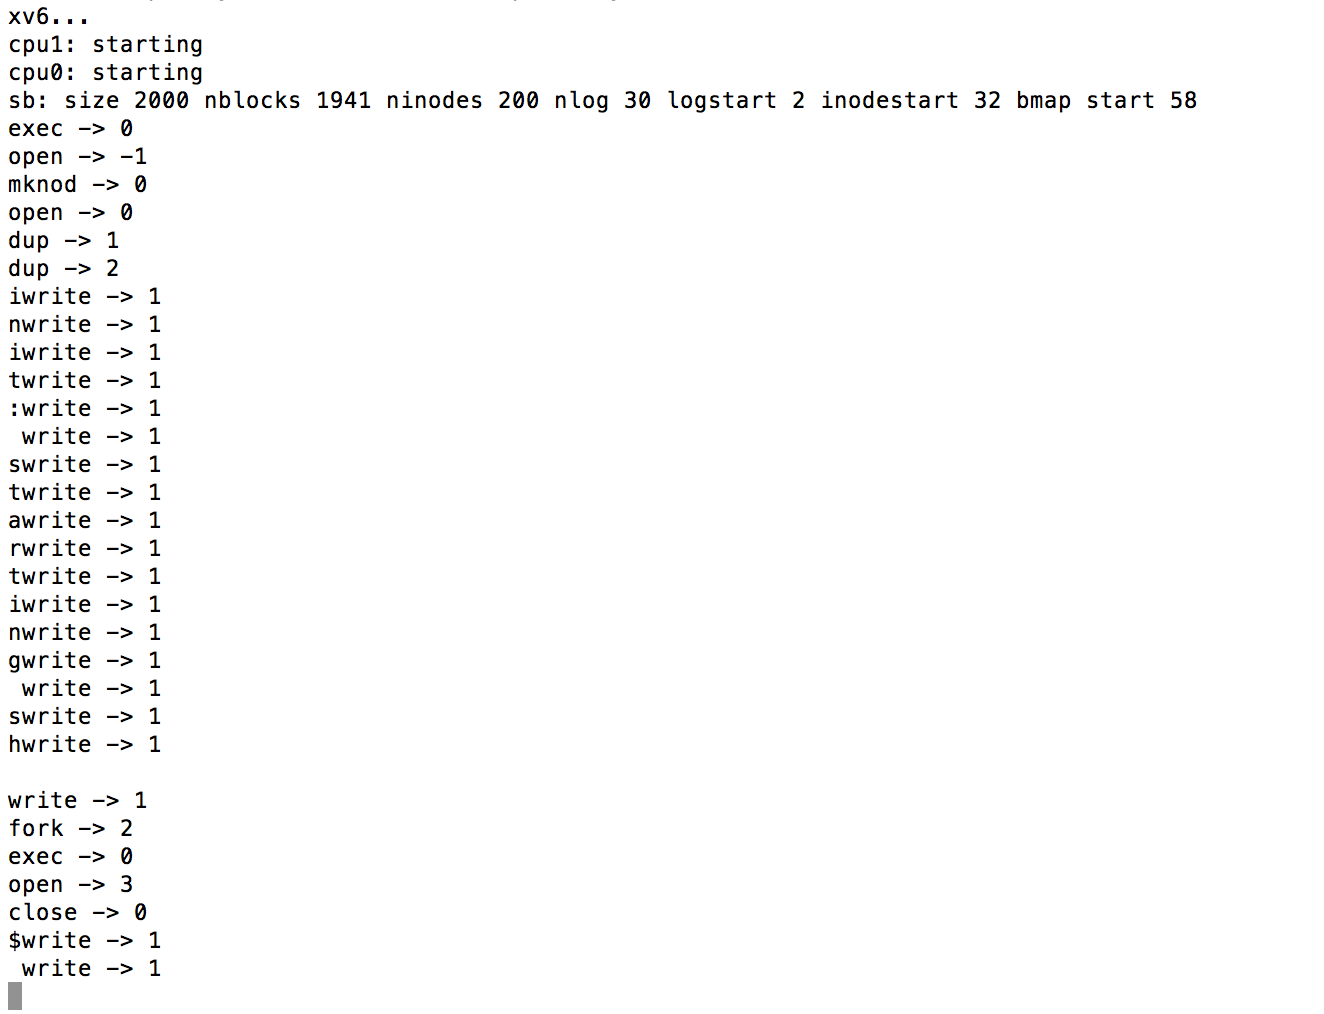
\includegraphics[width=0.8\linewidth]{sys-trace.png}
\caption[Syscall Trace]{System Call Tracing Facility}
\label{fig:syscalltrace}
\end{figure}
	
	The system call trace correctly displays invoked system calls. The standard output is interleaved with the trace output. The output ``init: starting sh'' is printed by the {\tt init()} process ({\tt init.c}) and the ``\$'' is printed by the shell process ({\tt sh.c}).
	
	This test {\tt PASSES}.

\newpage	
	\subsection*{Date System Call and User Command}
	I am going to use the {\tt date} command to test both the {\tt date()} system call and date command, as I can't directly invoke a system call from the shell. My testing will invoke my {\tt date} command in xv6 and then invoke the corresponding Linux {\tt date} command and see if the former closely matches the latter. 
	
\begin{figure}[h!]
\centering
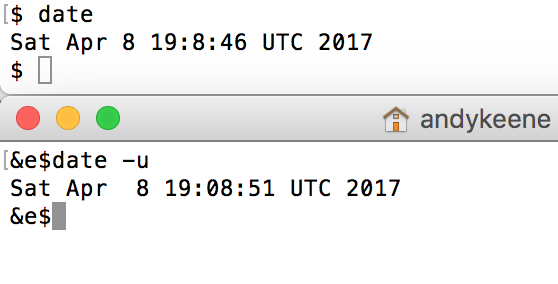
\includegraphics[width=0.4\linewidth]{date.png}
\caption[Date test]{Date Test}
\label{fig:datetest}
\end{figure}	
	
	The output from my {\tt date} command closely matches the output of the Linux {\tt date} command, except for a slight discrepancy in the number of seconds. This discrepancy is expected as it takes non-zero time to exit xv6. This test shows that the {\tt date} command works correctly, along with the date system call, since the command prints out all of the information extracted by the system call. Note also that the {\tt date} command on xv6, unlike {\tt date} on Linux, does \emph{not} print leading zeroes (see line 32 in {\tt date.c}); thus a further discrepancy in the output is due to {\tt date.c}'s implementation, but not the system call itself.
	
	This test {\tt PASSES}.
	
	\subsection*{control--p and Elapsed Time}
	The test for these will be split into two phases. My first test will show that control--p is outputting the correct information, while my second test will use the first test to show that the elapsed time is correct. \\
	
	\noindent Here is the output of the first test:

\begin{figure}[h]
\centering
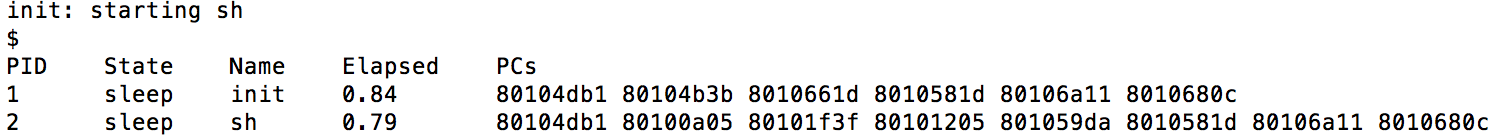
\includegraphics[width=0.8\linewidth]{ctrl-p-test1.png}
\caption[ctl-p test]{Control--p Test}
\label{fig:ctl-p_1}
\end{figure}	
	
	 The control--p output indicates that there are two processes running in xv6. This is correct. The first process is the initial process, here named ``init'', with a PID of 1. The second process is the shell, named ``sh'', with a PID of 2 (as it is the second process created). Note that the PCs appear to be correct, as they correspond to valid addresses in the kernel.asm file and the code for printing this information was not modified. 
	
	This sub-test {\tt PASSES}. 

\newpage
	For the second test, I will restart the kernel, and then press control--p several times, each press being within one second of the other. The results are shown below:

\begin{figure}[h!]
\centering
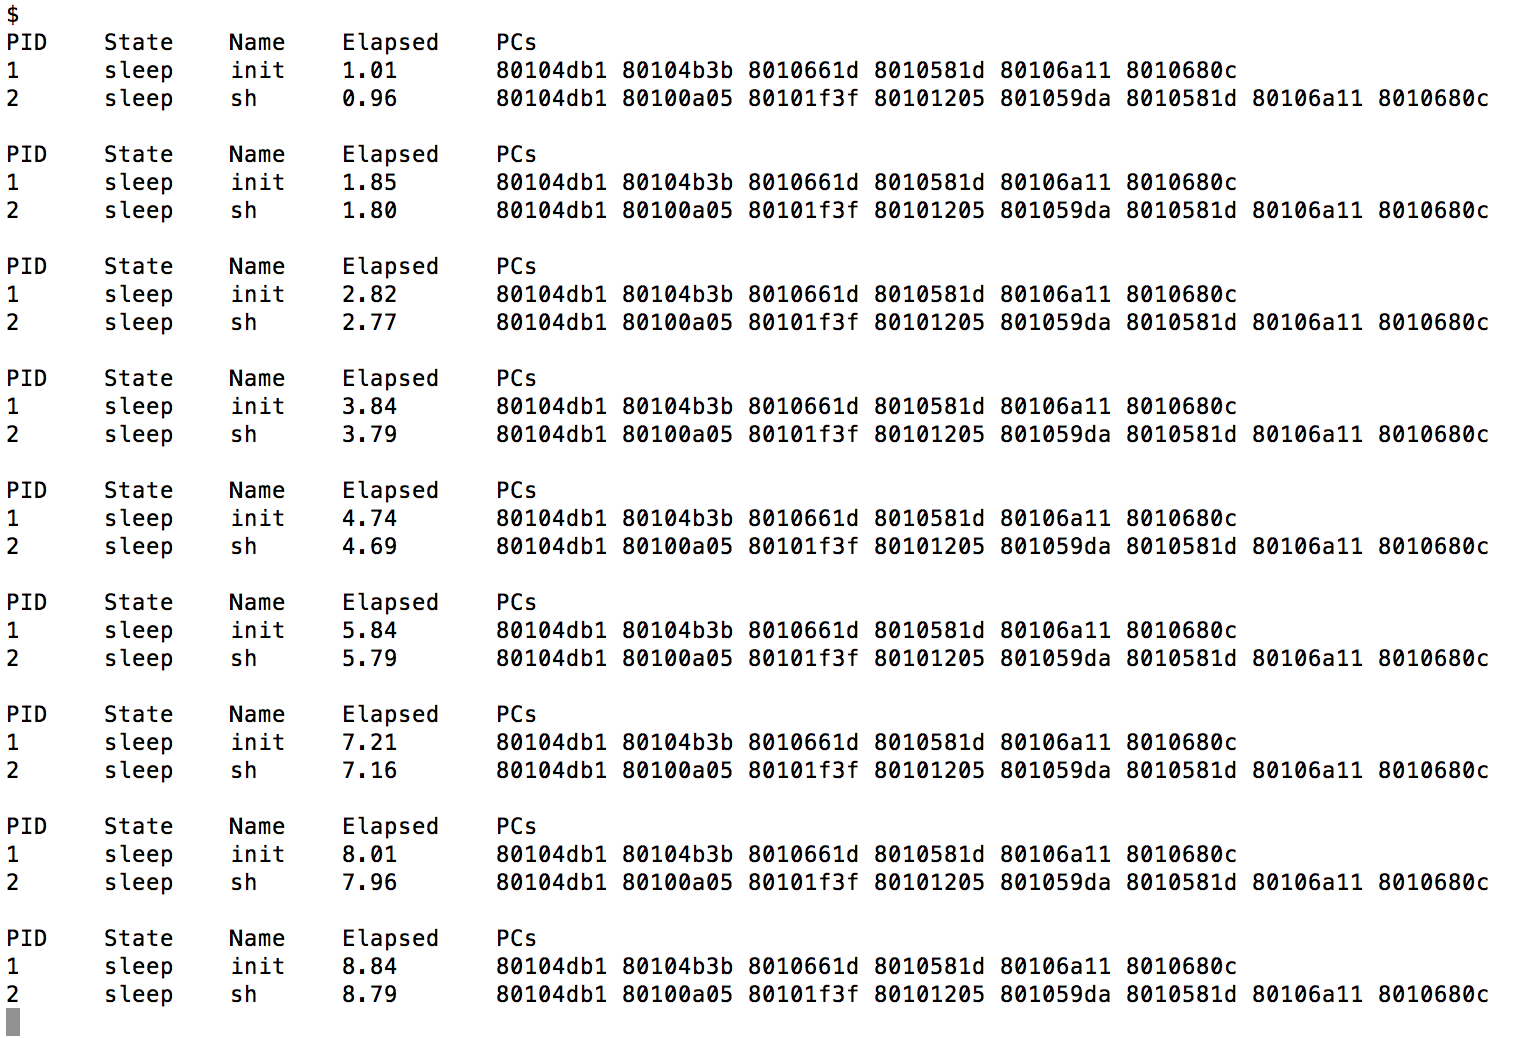
\includegraphics[width=0.8\linewidth]{ctrl-p-test2.png}
\caption[elapsed time]{Elapsed Time Test}
\label{fig:elapsed}
\end{figure}	
	
	The elapsed time for the  {\tt init} process is 0.05 seconds higher than that of the {\tt sh} process in all outputs. This makes sense as {\tt init} starts before {\tt sh}. Also, note that the elapsed times are steadily increasing by about one second with the same 0.05 second difference between {\tt init} and {\tt sh} and that leading zeros are printed for the hundredths of a second component of the time.
		
	This sub-test {\tt PASSES}.
	
	Because all sub-tests passed, this test {\tt PASSES}. \\

\end{document}